\externaldocument{implementation.tex}
\externaldocument{theory.tex}

\chapter{Výpočetní experimenty}
V této části práce jsou provedeny samotné výpočetní experimenty pomocí programu HullSolver. Experimenty byly provedeny na sadě různě komplikovaných benchmarkových problémů, z nichž část byla vymyšlena pro potřeby otestování implementace a část byla převzata z databáze polynomiálních problémů dostupné na adrese {\url{http://homepages.math.uic.edu/~jan/demo.html}.

Experimenty byly provedeny tak, že pro každou heuristiku uvedenou v~\ref{ch:usedHeuristics} byl spuštěn test se všemi dostupnými testovacími soubory a výsledky byly zaznamenány do tabulky. Použitá hodnota parametru \verb|eps| z kapitoly~\ref{ch:algorithms} byla 0,001.


\section{Testovací prostředí}
Veškeré experimenty s~programem HullSolver byly provedeny na~počítači s~operačním systémem MS Windows 10 Pro 64-bit v~běhovém prostředí .NET~4.6.1 v~následující hardwarové konfiguraci:

\begin{itemize}
\item Intel Core i5-4570 3,2~GHz (4 jádra)
\item 8~GB RAM DDR3 1600~MHz
\item nVidia GeForce GTX970
\end{itemize}

\section{Testovací úlohy}

Následuje seznam testovacích úloh s~krátkým popisem a údajem o~počtu primitivních podmínek. Úlohy převzaté z~databáze zmíněné výše jsou označeny hvězdičkou (*):

\begin{itemize}
    \item \emph{conform1*} - soustava tří polynomiálních rovnic stupně 3 o třech neznámých (24 podmínek),
    \item \emph{mickey*} - soustava dvou polynomiálních rovnic stupně 2 o dvou neznámých (6 podmínek),
    \item \emph{minus} - testovací rovnice pro ověření správnosti algoritmu $10(x - x + x - x + x - x + x) = 100$ (7 podmínek),
    \item \emph{polyn1} - rovnice $x^4 - 20x^2 + 64 = 0$ (4 podmínky),
    \item \emph{polyn2} - rovnice $x^3 - 2x = 0$ (4 podmínky),
    \item \emph{quadfor2*} - soustava čtyř rovnic stupně 3 o čtyřech neznámých (14 podmínek),
    \item \emph{solotarev*} - soustava čtyř rovnic stupně 2 o čtyřech neznámých (16 podmínek),
    \item \emph{wright*} - soustava pěti rovnic stupně 2 o pěti neznámých (26 podmínek).
\end{itemize}

Tabulky s~výsledky jsou uvedeny v~kapitole~\ref{ch:resultTables}. V těchto tabulkách jsou uvedeny naměřené hodnoty pro indikátory z~kapitoly \ref{ch:indicators}, přičemž jsou kvůli omezené šířce stránky následovně zkráceny názvy některých sloupců:


\begin{itemize}
    \item \# půlení - počet rozpůlení řešení,
    \item \# zúžení - celkový počet zúžení všech domén dohromady,
    \item poměr objemu - poměr objemu nejmenšího nalezeného boxu ku~objemu původního CSP.
\end{itemize}

O~kapitolu dále (\ref{ch:charts}) jsou k~nalezení grafy vykreslené na~základě dat z~tabulek. Tyto grafy jsou využity pro snazší porovnání heuristik.


\section{Tabulky}
\label{ch:resultTables}


\begin{table}[H]
\centering
\begin{tabular}{lrrrr}
\hline
problém & \# půlení & \# zúžení & poměr objemu & čas (s) \\ \hline
conform1 & 16 & 12441 & 6.777e-10 & 0.5688 \\
mickey & 30 & 227 & 5.722e-11 & 0.0462 \\
minus & 42 & 816 & 0.0009277 & 0.0554 \\
polyn1 & 35 & 645 & 0.0007813 & 0.0458 \\
polyn2 & 15 & 146 & 2.278e-38 & 0.0417 \\
quadfor2 & 89 & 3772 & 6.248e-17 & 0.1432 \\
solotarev & 99 & 15162 & 1.489e-15 & 0.6056 \\
wright & 2286 & 96850 & 3.458e-19 & 4.8842 \\
\end{tabular}
\caption{Výsledky pro heuristiku \emph{rand}}
\label{rand}
\end{table}



\begin{table}[H]
\centering
\begin{tabular}{lrrrr}
\hline
problém & \# půlení & \# zúžení & poměr objemu & čas (s) \\ \hline
conform1 & 16 & 8185 & 6.777e-10 & 0.3547 \\
mickey & 30 & 224 & 5.722e-11 & 0.0443 \\
minus & 42 & 760 & 0.0009277 & 0.0483 \\
polyn1 & 35 & 608 & 0.0007813 & 0.0463 \\
polyn2 & 15 & 131 & 0.0007813 & 0.0382 \\
quadfor2 & 89 & 3495 & 6.248e-17 & 0.1377 \\
solotarev & 95 & 11728 & 1.489e-15 & 0.5022 \\
wright & 2286 & 93533 & 3.458e-19 & 4.2201 \\
\end{tabular}
\caption{Výsledky pro heuristiku \emph{fifo}}
\label{fifo}
\end{table}



\begin{table}[H]
\centering
\begin{tabular}{lrrrr}
\hline
problém & \# půlení & \# zúžení & poměr objemu & čas (s) \\ \hline
conform1 & 16 & 7995 & 6.777e-10 & 0.6239 \\
mickey & 30 & 240 & 5.722e-11 & 0.0433 \\
minus & 42 & 767 & 0.0009277 & 0.0538 \\
polyn1 & 35 & 608 & 0.0007813 & 0.0467 \\
polyn2 & 15 & 125 & 0.0007813 & 0.0390 \\
quadfor2 & 89 & 3126 & 6.248e-17 & 0.1771 \\
solotarev & 95 & 9493 & 1.489e-15 & 0.6660 \\
wright & 2286 & 88059 & 3.458e-19 & 8.4097 \\
\end{tabular}
\caption{Výsledky pro heuristiku \emph{dom-first}}
\label{dom-first}
\end{table}



\begin{table}[H]
\centering
\begin{tabular}{lrrrr}
\hline
problém & \# půlení & \# zúžení & poměr objemu & čas (s) \\ \hline
conform1 & 16 & 10194 & 6.777e-10 & 0.7317 \\
mickey & 30 & 225 & 5.722e-11 & 0.0435 \\
minus & 42 & 800 & 0.0009277 & 0.0529 \\
polyn1 & 35 & 606 & 0.0007813 & 0.0506 \\
polyn2 & 15 & 128 & 0.0007813 & 0.0465 \\
quadfor2 & 89 & 3552 & 6.248e-17 & 0.2243 \\
solotarev & 95 & 20800 & 1.489e-15 & 1.2040 \\
wright & 2286 & 108977 & 3.458e-19 & 10.4618 \\
\end{tabular}
\caption{Výsledky pro heuristiku \emph{nondom-first}}
\label{nondom-first}
\end{table}



\begin{table}[H]
\centering
\begin{tabular}{lrrrr}
\hline
problém & \# půlení & \# zúžení & poměr objemu & čas (s) \\ \hline
conform1 & 16 & 23673 & 6.777e-10 & 1.5826 \\
mickey & 30 & 255 & 5.722e-11 & 0.0513 \\
minus & 42 & 826 & 0.0009277 & 0.0639 \\
polyn1 & 35 & 646 & 0.0007813 & 0.0541 \\
polyn2 & 15 & 127 & 0.0007813 & 0.0433 \\
quadfor2 & 89 & 6672 & 6.248e-17 & 0.3859 \\
solotarev & 95 & 162967 & 1.489e-15 & 11.7988 \\
wright & 2286 & 98378 & 3.458e-19 & 11.3865 \\
\end{tabular}
\caption{Výsledky pro heuristiku \emph{max-right-cand}}
\label{max-right-cand}
\end{table}



\begin{table}[H]
\centering
\begin{tabular}{lrrrr}
\hline
problém & \# půlení & \# zúžení & poměr objemu & čas (s) \\ \hline
conform1 & 16 & 23306 & 6.777e-10 & 1.4782 \\
mickey & 30 & 217 & 5.722e-11 & 0.0481 \\
minus & 42 & 769 & 0.0009277 & 0.0668 \\
polyn1 & 35 & 638 & 0.0007813 & 0.0525 \\
polyn2 & 15 & 478 & 9.243e-35 & 0.0479 \\
quadfor2 & 169 & 66938 & 6.248e-17 & 3.6092 \\
solotarev & 116 & 540970 & 3.669e-16 & 34.8202 \\
wright & 2286 & 96594 & 3.458e-19 & 9.6712 \\
\end{tabular}
\caption{Výsledky pro heuristiku \emph{min-right-cand}}
\label{min-right-cand}
\end{table}



\begin{table}[H]
\centering
\begin{tabular}{lrrrr}
\hline
problém & \# půlení & \# zúžení & poměr objemu & čas (s) \\ \hline
conform1 & 16 & 15528 & 6.777e-10 & 1.3386 \\
mickey & 30 & 260 & 5.722e-11 & 0.0758 \\
minus & 42 & 809 & 0.0009277 & 0.0838 \\
polyn1 & 35 & 647 & 0.0007813 & 0.0563 \\
polyn2 & 15 & 130 & 0.0007813 & 0.0488 \\
quadfor2 & 169 & 7682 & 6.248e-17 & 0.5212 \\
solotarev & 95 & 136896 & 1.489e-15 & 9.3976 \\
wright & 2286 & 119420 & 3.458e-19 & 13.4664 \\
\end{tabular}
\caption{Výsledky pro heuristiku \emph{large-int-first}}
\label{large-int-first}
\end{table}



\begin{table}[H]
\centering
\begin{tabular}{lrrrr}
\hline
problém & \# půlení & \# zúžení & poměr objemu & čas (s) \\ \hline
conform1 & 16 & 36655 & 6.777e-10 & 2.2830 \\
mickey & 30 & 215 & 5.722e-11 & 0.0435 \\
minus & 42 & 708 & 0.0009277 & 0.0559 \\
polyn1 & 35 & 643 & 0.0007813 & 0.0486 \\
polyn2 & 15 & 477 & 9.243e-35 & 0.0451 \\
quadfor2 & 169 & 159 & 6.248e-17 & 0.0458 \\
solotarev & 116 & 118221 & 3.669e-16 & 8.2039 \\
wright & 2286 & 86619 & 3.458e-19 & 9.3518 \\
\end{tabular}
\caption{Výsledky pro heuristiku \emph{small-int-first}}
\label{small-int-first}
\end{table}



\begin{table}[H]
\centering
\begin{tabular}{lrrrr}
\hline
problém & \# půlení & \# zúžení & poměr objemu & čas (s) \\ \hline
conform1 & 16 & 15528 & 6.777e-10 & 1.0341 \\
mickey & 30 & 253 & 5.722e-11 & 0.0457 \\
minus & 42 & 809 & 0.0009277 & 0.0560 \\
polyn1 & 35 & 644 & 0.0007813 & 0.0495 \\
polyn2 & 15 & 137 & 0.0007813 & 0.0399 \\
quadfor2 & 169 & 7696 & 6.248e-17 & 0.4336 \\
solotarev & 95 & 95883 & 1.489e-15 & 6.5600 \\
wright & 2286 & 127848 & 3.458e-19 & 15.9222 \\
\end{tabular}
\caption{Výsledky pro heuristiku \emph{shrunk-most-first}}
\label{shrunk-most-first}
\end{table}



\begin{table}[H]
\centering
\begin{tabular}{lrrrr}
\hline
problém & \# půlení & \# zúžení & poměr objemu & čas (s) \\ \hline
conform1 & 16 & 36041 & 6.777e-10 & 3.0409 \\
mickey & 30 & 221 & 5.722e-11 & 0.0445 \\
minus & 42 & 708 & 0.0009277 & 0.0585 \\
polyn1 & 35 & 630 & 0.0007813 & 0.0500 \\
polyn2 & 15 & 167 & 2.278e-38 & 0.0406 \\
quadfor2 & 89 & 33264 & 6.248e-17 & 1.6815 \\
solotarev & 116 & 361640 & 3.669e-16 & 23.1700 \\
wright & 2286 & 79055 & 3.458e-19 & 10.0826 \\
\end{tabular}
\caption{Výsledky pro heuristiku \emph{shrunk-least-first}}
\label{shrunk-least-first}
\end{table}



\begin{table}[H]
\centering
\begin{tabular}{lrrrr}
\hline
problém & \# půlení & \# zúžení & poměr objemu & čas (s) \\ \hline
conform1 & 16 & 8376 & 6.777e-10 & 3.1547 \\
mickey & 30 & 236 & 5.722e-11 & 0.0526 \\
minus & 42 & 767 & 0.0009277 & 0.0766 \\
polyn1 & 35 & 611 & 0.0007813 & 0.0523 \\
polyn2 & 15 & 125 & 0.0007813 & 0.0415 \\
quadfor2 & 89 & 3065 & 6.248e-17 & 0.5714 \\
solotarev & 95 & 8208 & 1.489e-15 & 2.2684 \\
wright & 2286 & 89847 & 3.458e-19 & 51.7957 \\
\end{tabular}
\caption{Výsledky pro heuristiku \emph{fail-first}}
\label{fail-first}
\end{table}



\begin{table}[H]
\centering
\begin{tabular}{lrrrr}
\hline
problém & \# půlení & \# zúžení & poměr objemu & čas (s) \\ \hline
conform1 & 16 & 11787 & 6.777e-10 & 0.6058 \\
mickey & 30 & 252 & 5.722e-11 & 0.0426 \\
minus & 42 & 760 & 0.0009277 & 0.0507 \\
polyn1 & 35 & 639 & 0.0007813 & 0.0465 \\
polyn2 & 15 & 130 & 0.0007813 & 0.0411 \\
quadfor2 & 89 & 3502 & 6.248e-17 & 0.1508 \\
solotarev & 95 & 10434 & 1.489e-15 & 0.5193 \\
wright & 2286 & 141514 & 3.458e-19 & 6.9660 \\
\end{tabular}
\caption{Výsledky pro heuristiku \emph{prefer-add}}
\label{prefer-add}
\end{table}



\begin{table}[H]
\centering
\begin{tabular}{lrrrr}
\hline
problém & \# půlení & \# zúžení & poměr objemu & čas (s) \\ \hline
conform1 & 16 & 6777 & 6.777e-10 & 0.3781 \\
mickey & 30 & 242 & 5.722e-11 & 0.0438 \\
minus & 42 & 760 & 0.0009277 & 0.0519 \\
polyn1 & 35 & 605 & 0.0007813 & 0.0452 \\
polyn2 & 15 & 127 & 0.0007813 & 0.0391 \\
quadfor2 & 89 & 3519 & 6.248e-17 & 0.1817 \\
solotarev & 95 & 8526 & 1.489e-15 & 0.4209 \\
wright & 2286 & 86273 & 3.458e-19 & 3.9737 \\
\end{tabular}
\caption{Výsledky pro heuristiku \emph{prefer-mult}}
\label{prefer-mult}
\end{table}







\section{Grafy}
\label{ch:charts}
\begin{figure}[H]
\centering
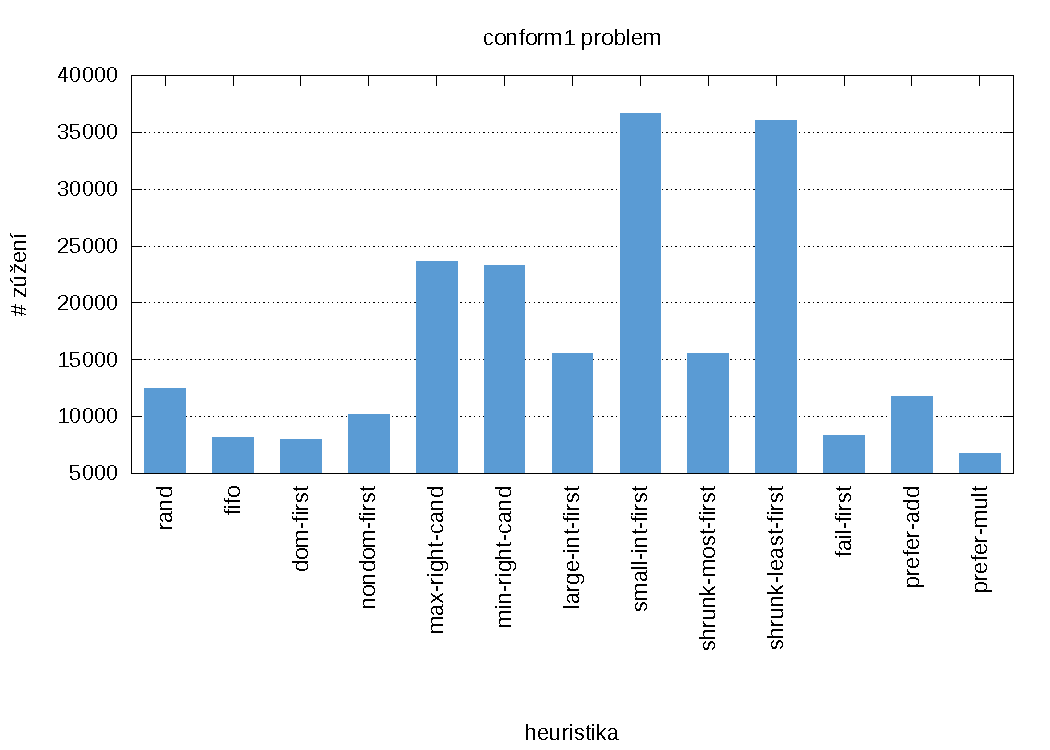
\includegraphics[scale=0.68]{chart/conform1_nar.pdf}
\caption{Porovnání heuristik pro problém \emph{conform1} podle počtu zúžení}
\end{figure}

\begin{figure}[H]
\centering
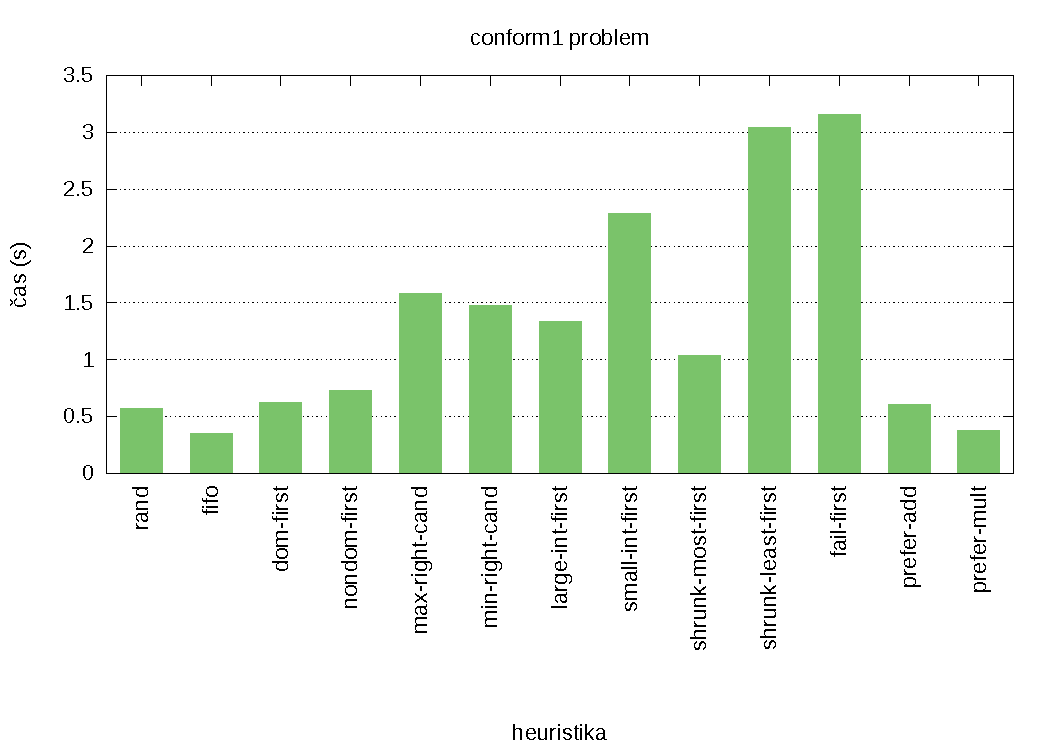
\includegraphics[scale=0.68]{chart/conform1_time.pdf}
\caption{Porovnání heuristik pro problém \emph{conform1} podle času}
\end{figure}

\begin{figure}[H]
\centering
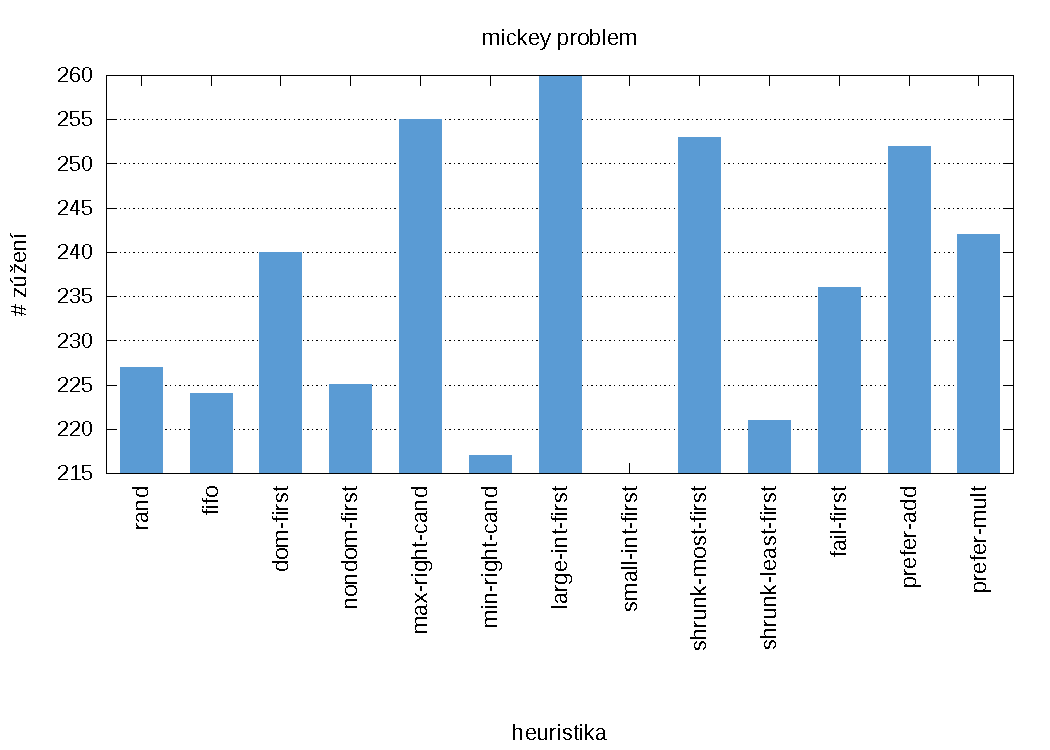
\includegraphics[scale=0.68]{chart/mickey_nar.pdf}
\caption{Porovnání heuristik pro problém \emph{mickey} podle počtu zúžení}
\end{figure}

\begin{figure}[H]
\centering
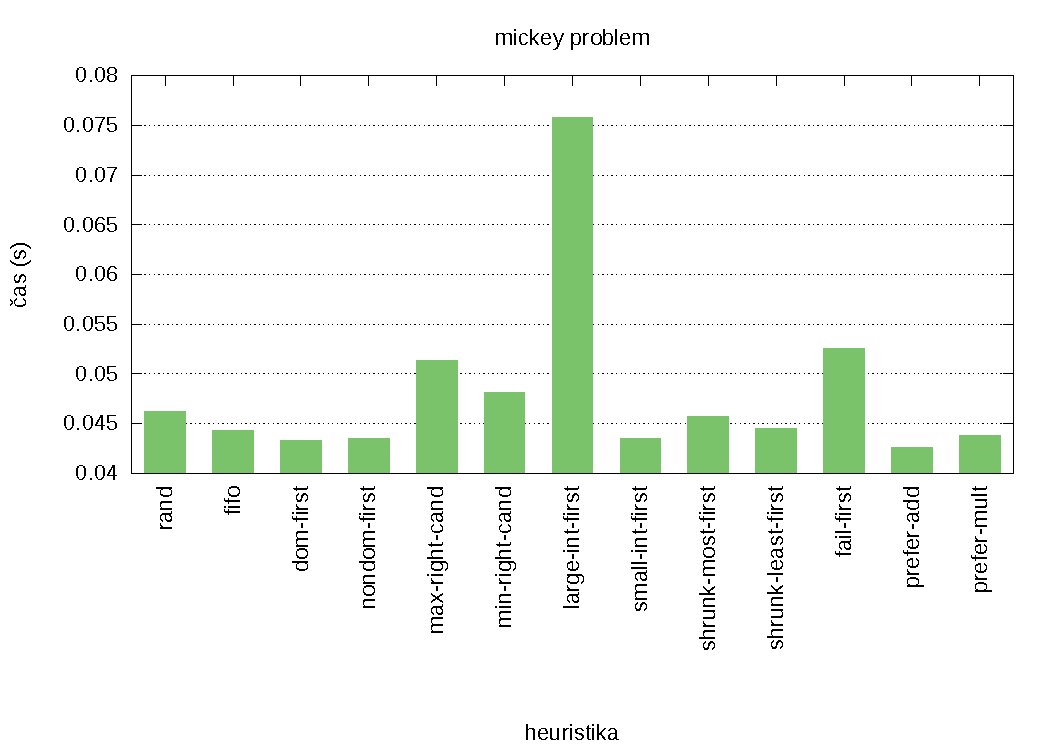
\includegraphics[scale=0.68]{chart/mickey_time.pdf}
\caption{Porovnání heuristik pro problém \emph{mickey} podle času}
\end{figure}



\begin{figure}[H]
\centering
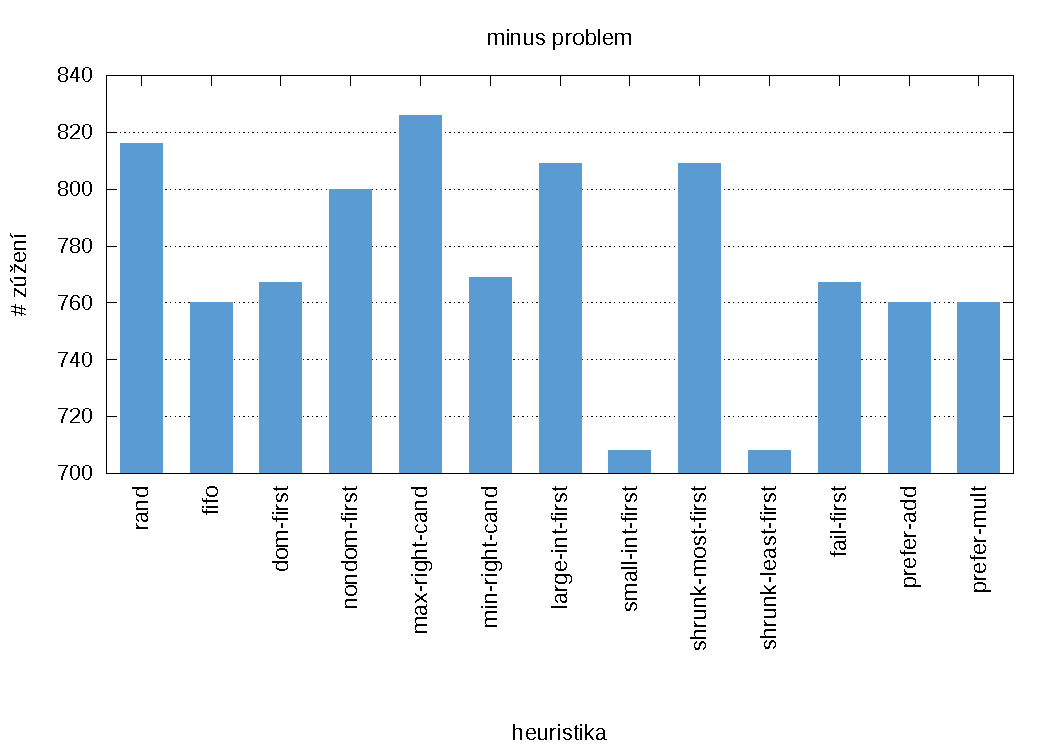
\includegraphics[scale=0.68]{chart/minus_nar.pdf}
\caption{Porovnání heuristik pro problém \emph{minus} podle počtu zúžení}
\end{figure}


\begin{figure}[H]
\centering
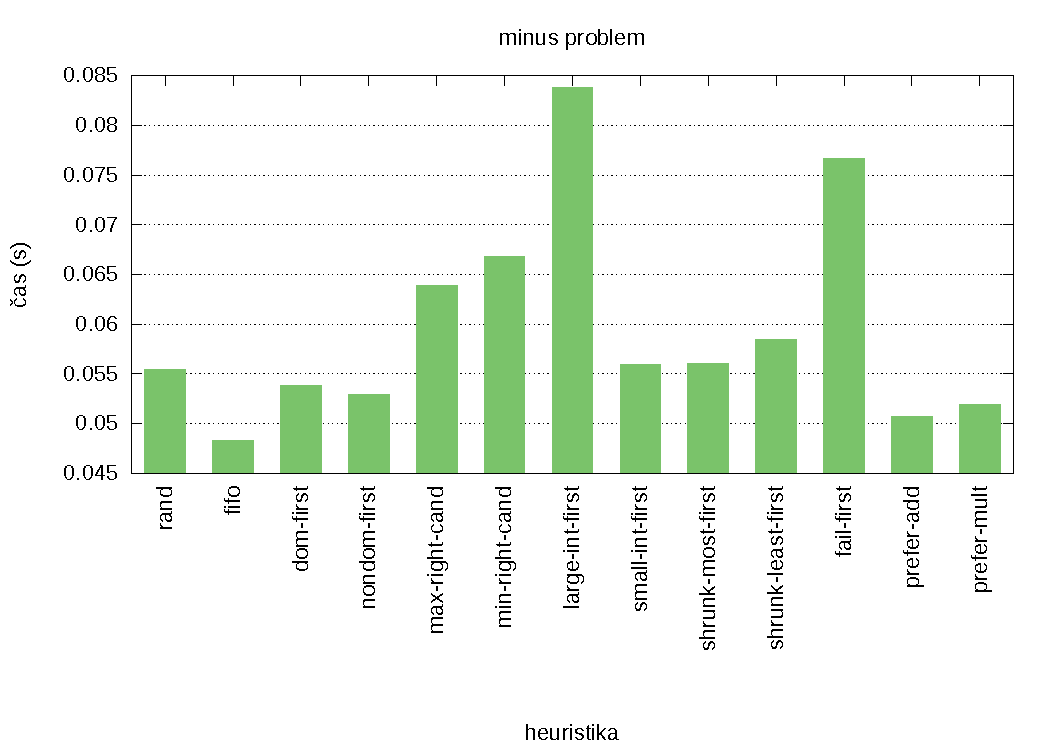
\includegraphics[scale=0.68]{chart/minus_time.pdf}
\caption{Porovnání heuristik pro problém \emph{minus} podle času}
\end{figure}

\begin{figure}[H]
\centering
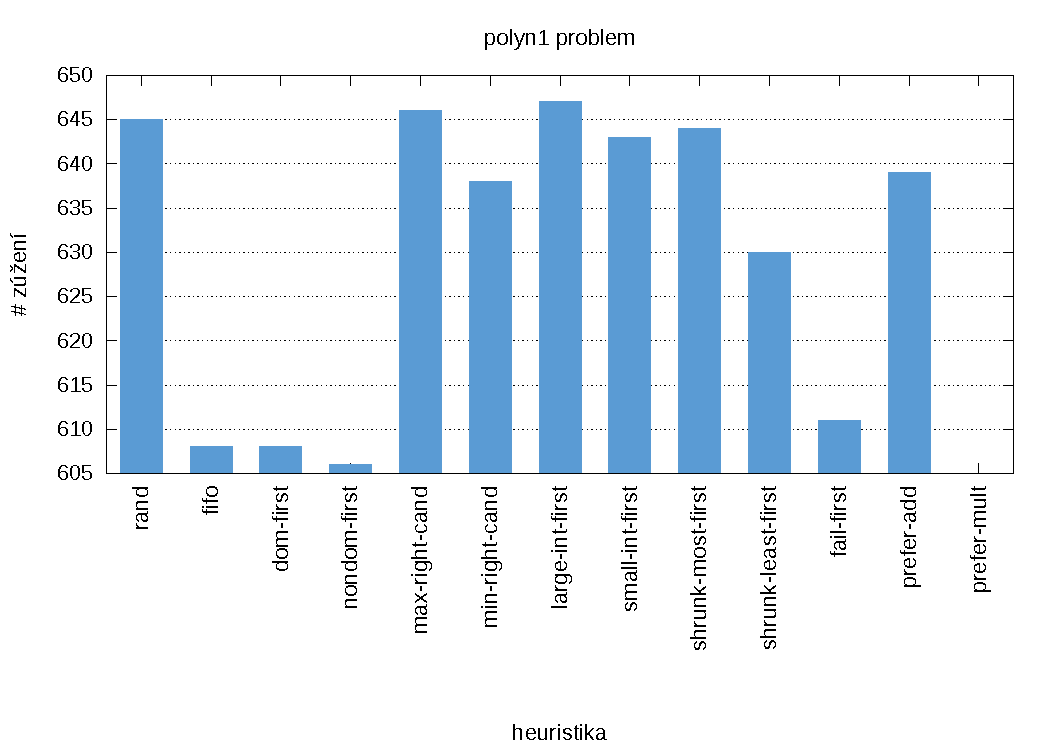
\includegraphics[scale=0.68]{chart/polyn1_nar.pdf}
\caption{Porovnání heuristik pro problém \emph{polyn1} podle počtu zúžení}
\end{figure}

\begin{figure}[H]
\centering
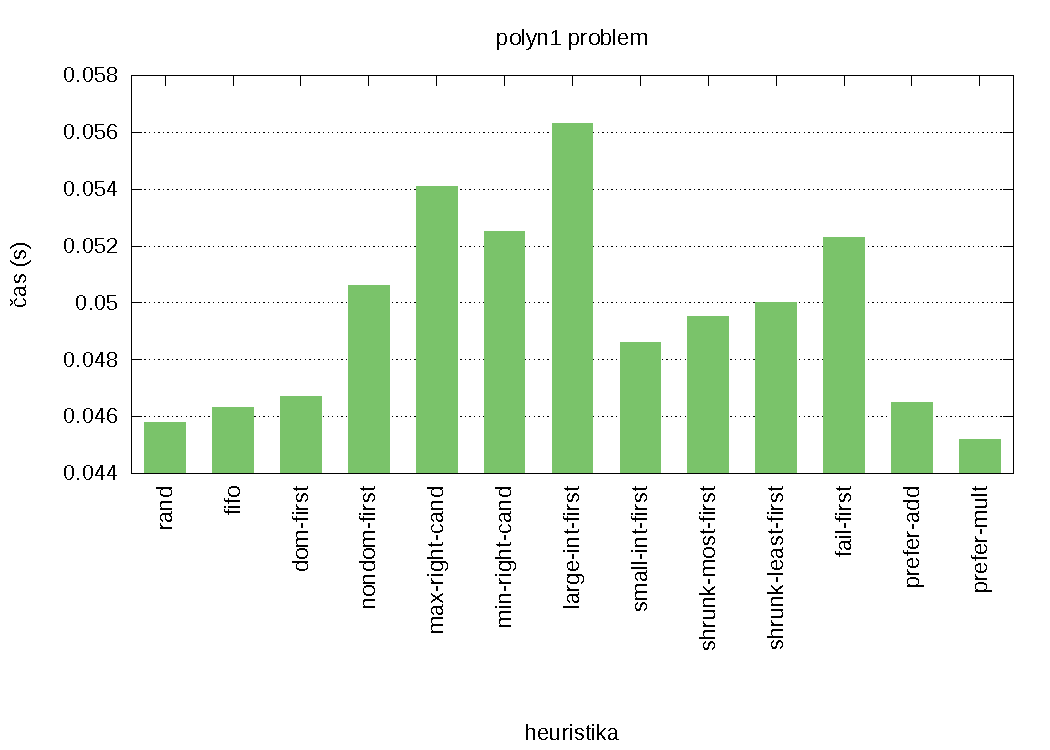
\includegraphics[scale=0.68]{chart/polyn1_time.pdf}
\caption{Porovnání heuristik pro problém \emph{polyn1} podle času}
\end{figure}

\begin{figure}[H]
\centering
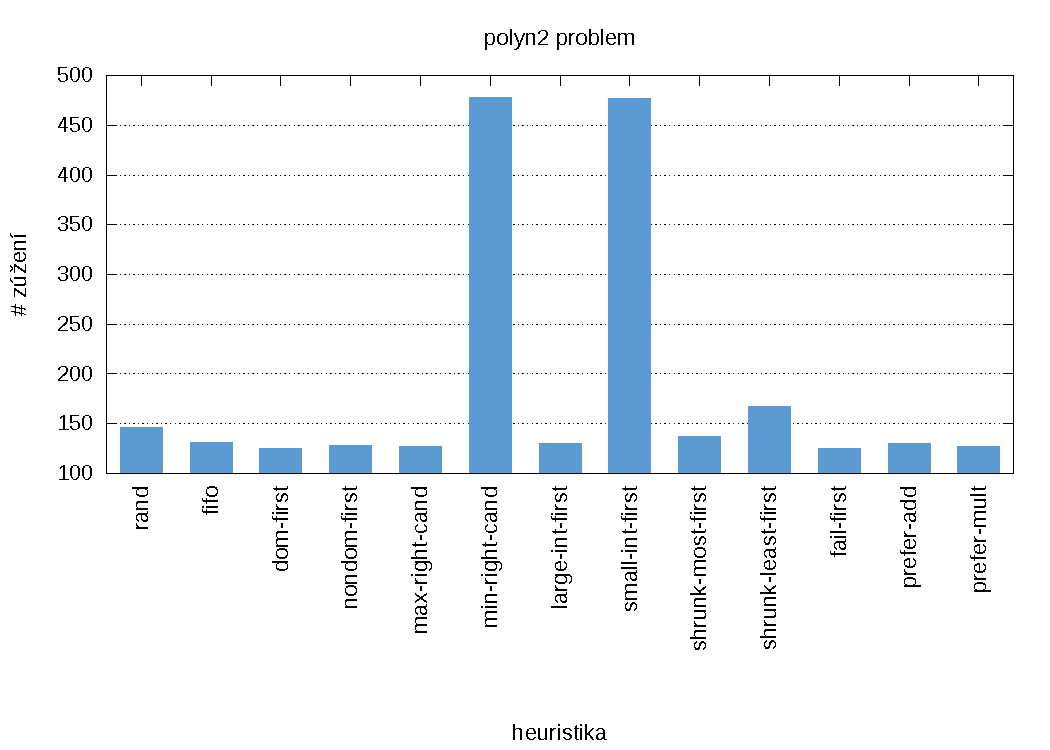
\includegraphics[scale=0.68]{chart/polyn2_nar.pdf}
\caption{Porovnání heuristik pro problém \emph{polyn2} podle počtu zúžení}
\end{figure}

\begin{figure}[H]
\centering
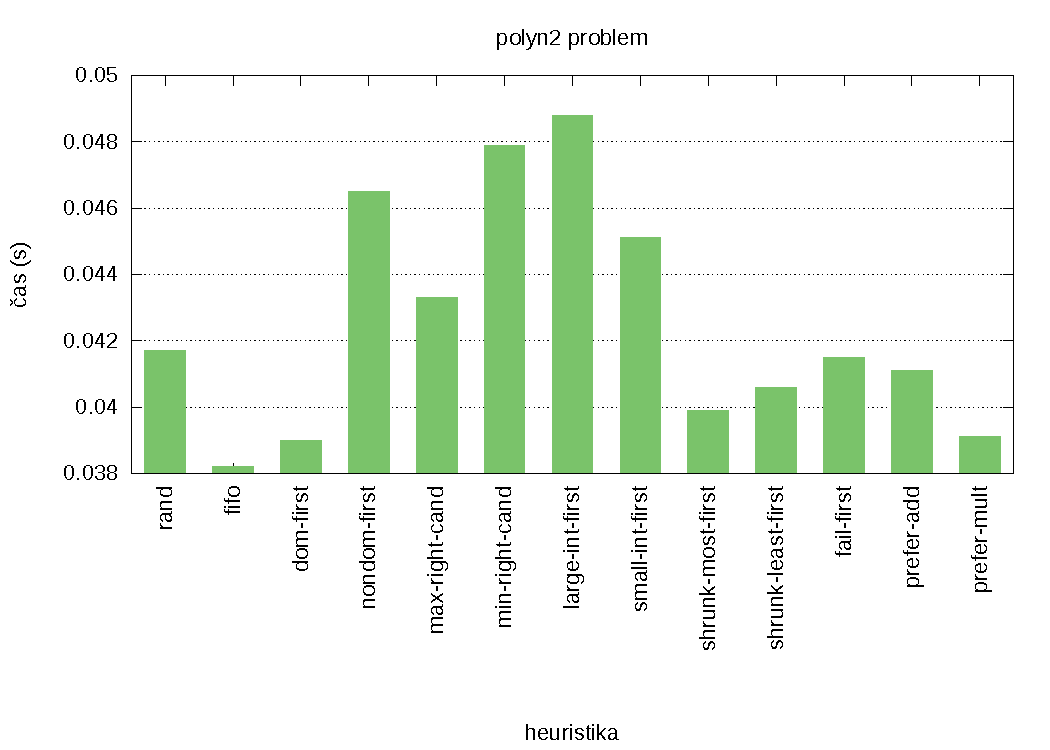
\includegraphics[scale=0.68]{chart/polyn2_time.pdf}
\caption{Porovnání heuristik pro problém \emph{polyn2} podle času}
\end{figure}

\begin{figure}[H]
\centering
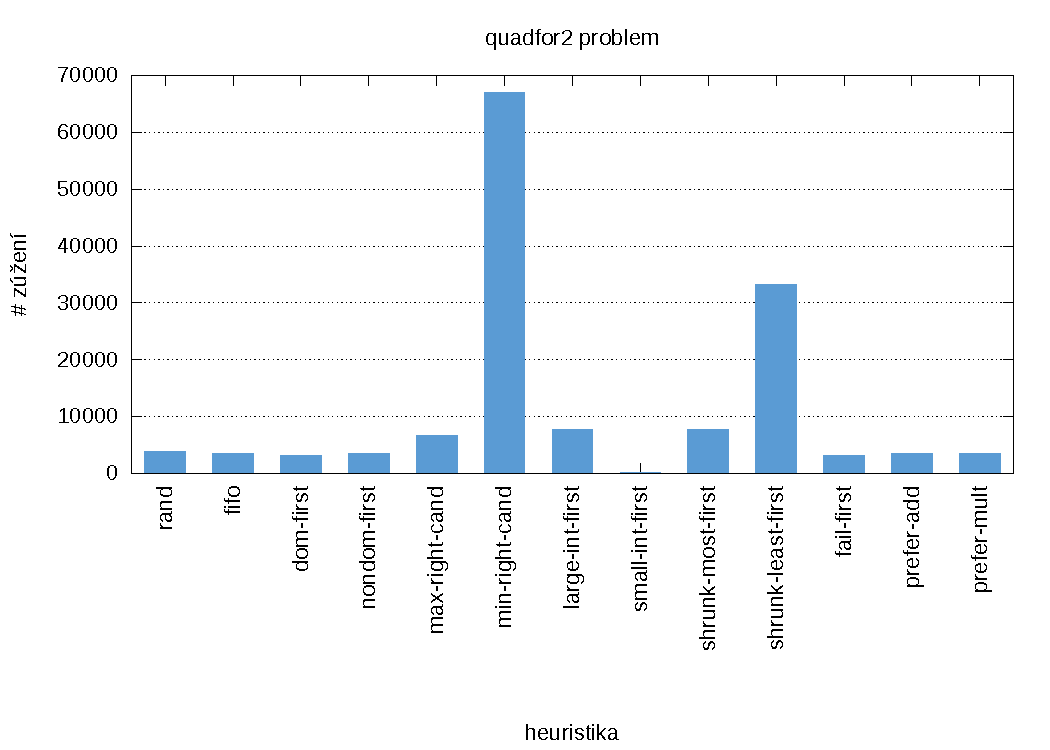
\includegraphics[scale=0.68]{chart/quadfor2_nar.pdf}
\caption{Porovnání heuristik pro problém \emph{quadfor2} podle počtu zúžení}
\end{figure}

\begin{figure}[H]
\centering
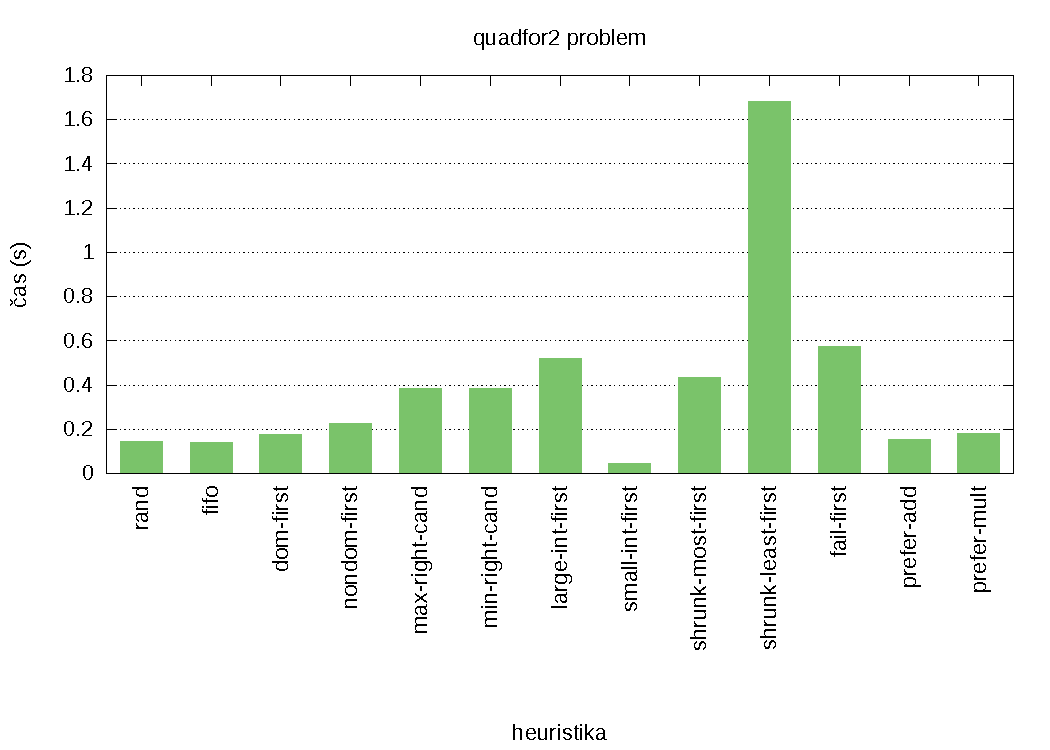
\includegraphics[scale=0.68]{chart/quadfor2_time.pdf}
\caption{Porovnání heuristik pro problém \emph{quadfor2} podle času}
\end{figure}

\begin{figure}[H]
\centering
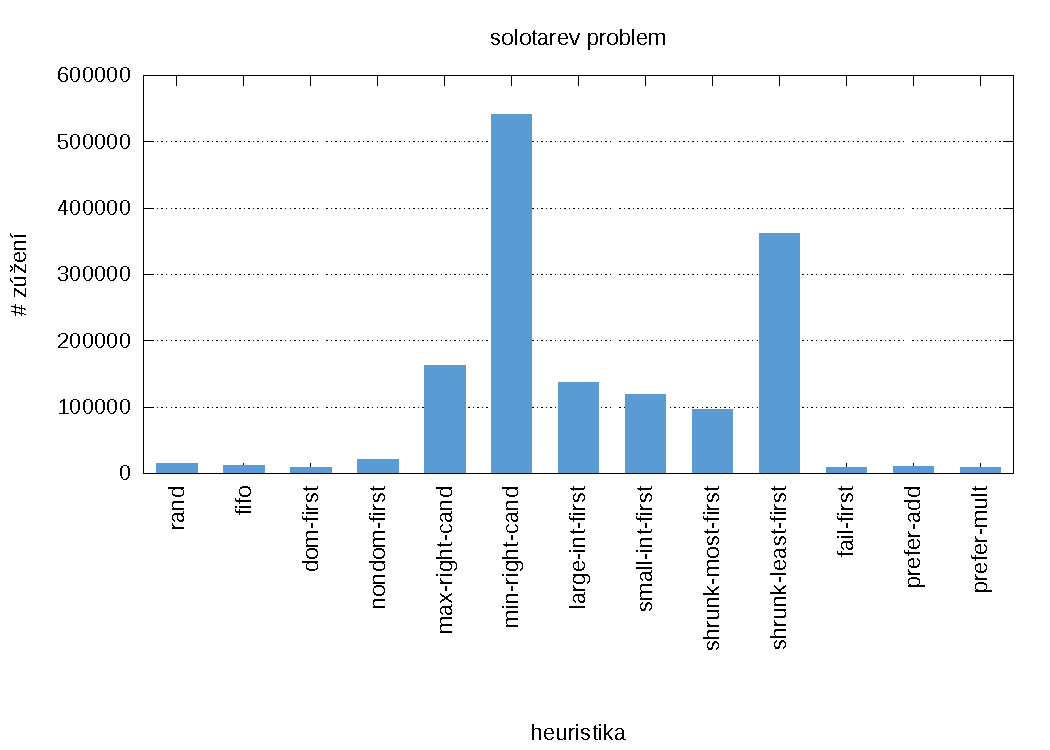
\includegraphics[scale=0.68]{chart/solotarev_nar.pdf}
\caption{Porovnání heuristik pro problém \emph{solotarev} podle počtu zúžení}
\end{figure}

\begin{figure}[H]
\centering
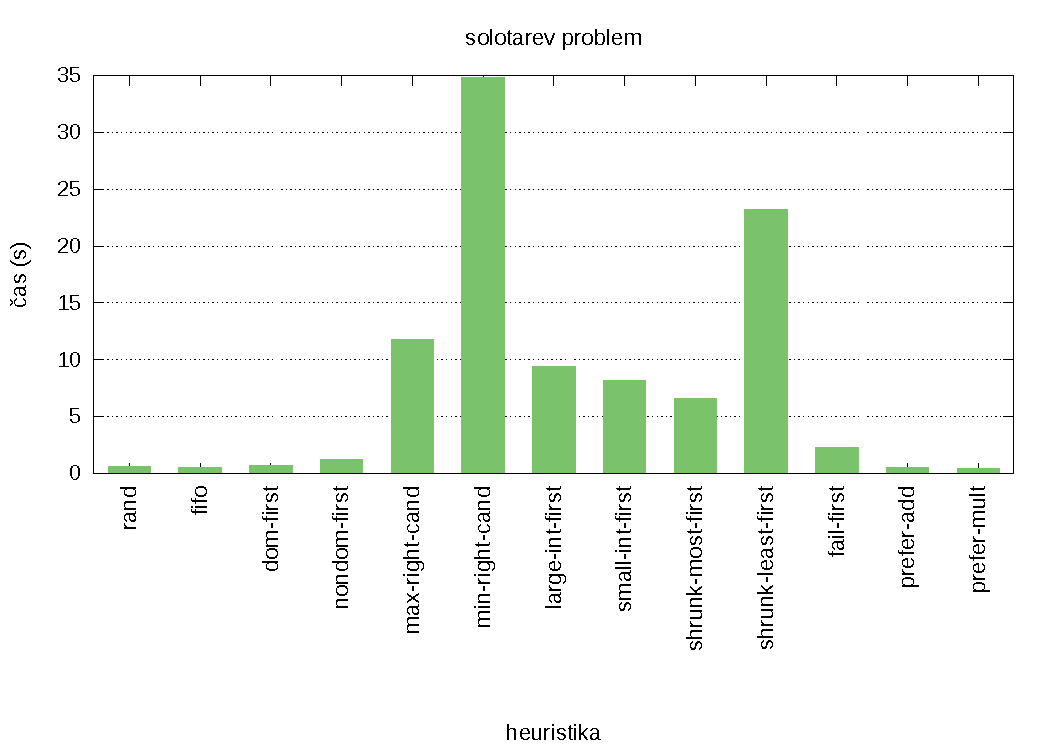
\includegraphics[scale=0.68]{chart/solotarev_time.pdf}
\caption{Porovnání heuristik pro problém \emph{solotarev} podle času}
\end{figure}

\begin{figure}[H]
\centering
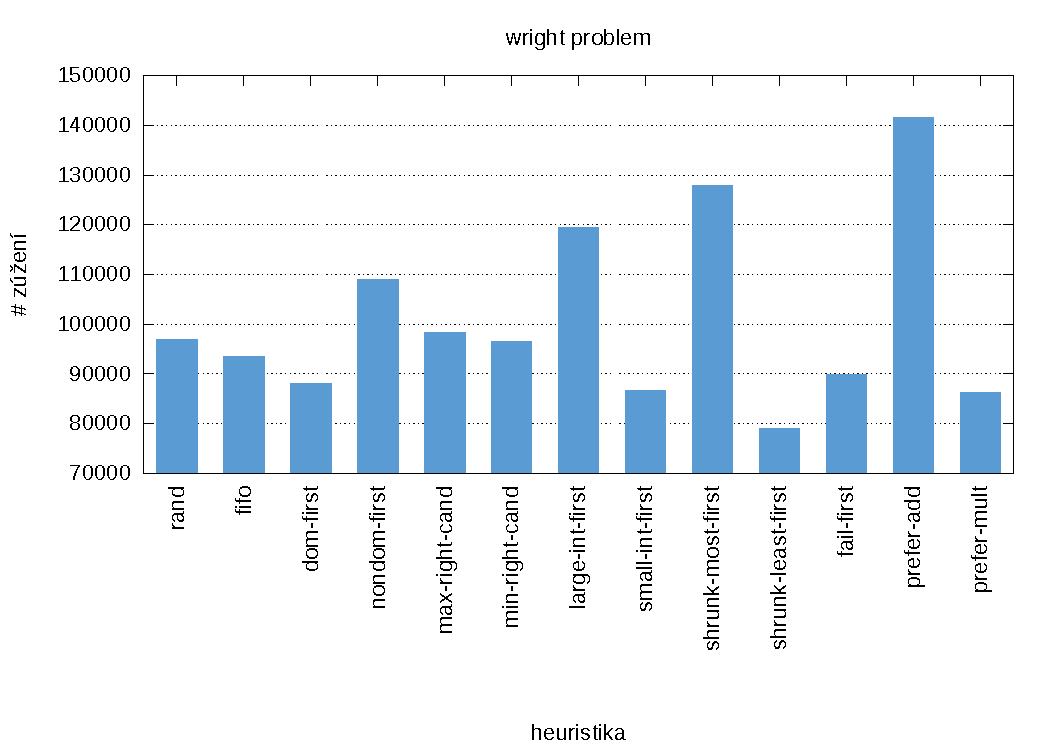
\includegraphics[scale=0.68]{chart/wright_nar.pdf}
\caption{Porovnání heuristik pro problém \emph{wright} podle počtu zúžení}
\end{figure}

\begin{figure}[H]
\centering
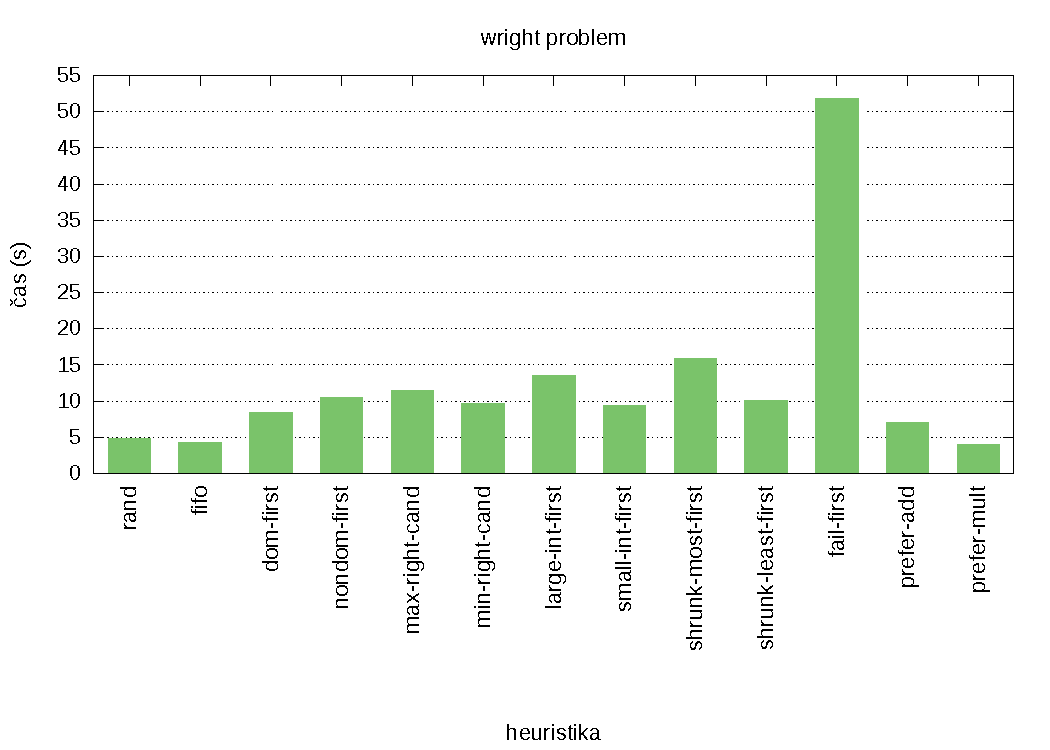
\includegraphics[scale=0.68]{chart/wright_time.pdf}
\caption{Porovnání heuristik pro problém \emph{wright} podle času}
\end{figure}


\section{Vyhodnocení výsledků}
Následující odstavce porovnávají heuristiky z~pohledu hodnot naměřených pro různé indikátory. Platí, že \uv{lepší} či \uv{dobrá} heuristika má tyto hodnoty nižší než \uv{horší} či \uv{špatná} heuristika.

V tabulkách výše je vidět, že se u~jednotlivých heuristik v~rámci jedné testovací úlohy příliš neměnily hodnoty ve~sloupcích \uv{\# půlení} a \uv{poměr objemu}. Bylo možné očekávat, že obě hodnoty budou ve~většině případů stejné - v~případě počtu půlení bude pravděpodobně na~vině fakt, že při půlení je proměnná, jejíž doména se bude půlit, vybírána metodou round-robin a~pořadí proměnné je při každém spuštění algoritmu stejné. Dojde tedy k~tomu, že algoritmus HC3 vždy zmenší problém, jak nejvíce dokáže (důležité je, že tohoto dosáhne nehledě na použitou heuristiku), poté se box rozpůlí podle proměnné (opět podle stejné proměnné nehledě na~použitou heuristiku) a toto se rekurzivně opakuje. Rozdílné hodnoty u~několika málo vstupů mohou být způsobeny nepřesným porovnáváním čísel s~plovoucí řádovou čárkou. Hodnoty ve~sloupci \uv{poměr objemu} se pro jeden problém většinou nemění, protože je při startu algoritmu pevně dáno, kolikrát se má objem počátečního boxu zmenšit (hodnota \verb|eps|).

Další indikátor, čas, je zobrazen v~grafech z~předchozí kapitoly. Heuristika \emph{fifo} (simuluje FIFO frontu a pouze v~čase $\mathcal{O}(1)$ vrátí první prvek ze~seznamu) dosahuje ve~srovnání s~ostatními heuristikami velmi dobrých výsledků, co se času týče, v~pěti z~osmi případů. To poukazuje na~skutečnost, že výpočet ostatních heuristik, které dvojici pro další zpracování vyhledávají v~celém seznamu v~čase $\mathcal{O}(n)$, zpomaluje běh programu.

Heuristikou nejvíce zpomalující běh programu se ukázala být heuristika \emph{large-int-first} (výrazně pomalejší než ostatní byla v~polovině případů), která vrací dvojici, jejíž proměnná má nejširší doménu. To je logické, protože cílem algoritmu je zúžit domény dominantních proměnných pod určitou mez a~při výběru vždy té nejširší domény se program může zdržovat se zužováním domén, které nemusí být nutně potřeba zúžit.

I~výsledky pro poslední indikátor, počet zúžení, jsou zobrazeny v~grafech. Zde již výsledky nejsou tak jasné, jako v~případě času. Lze říct, že nejlepších výsledků dosáhla heuristika \emph{prefer-mult}, která byla ve dvou případech znatelně lepší než ostatní a~ve dvou případech přibližně stejně dobrá jako ostatní. Tato heuristika vybírá první dvojici, jejíž omezující podmínka obsahuje operaci násobení. Při bližším prozkoumání testovacích úloh si lze všimnout, že omezující podmínky problémů, u~kterých tato heuristika zafungovala dobře, jsou z~více než poloviny tvořeny podmínkami s~operací násobení. Opačný jev, tedy že by heuristika \emph{prefer-add} byla lepší než ostatní u~problémů s~majoritním zastoupením podmínek se sčítáním/násobením, nebyl pozorován.

Nejhorších výsledků z~pohledu počtu zúžení dosáhla u~složitějších úloh (\emph{quadfor2}, \emph{solotarev}) heuristika \emph{min-right-cand}, v~jednom případě byla nejhorší i~\emph{max-right-cand}. Velikost pravé meze domény tedy zřejmě neposkytuje žádnou užitečnou informaci, která by zefektivnila průběh řešení. Špatných výsledků dosáhla také heuristika \emph{large-int-first}, ze stejného důvodu jako u~času.

Algoritmus využívající heuristiku \emph{prefer-mult}, který by ukládal dvojice do seznamu již optimálně seřazené tak, aby je stačilo ze začátku seznamu v~čase $\mathcal{O}(1)$ odebírat, by mohl u~některého typu úloh dosahovat velmi dobrých výsledků. Naopak jistě se nevyplatí používat heuristiky, které se rozhodují podle velikosti jedné z mezí, nebo takové, které preferují největší domény. Otestování algoritmu na několika desítkách úloh by ale mohlo přinést jiné výsledky. Je také možné, že existují i o mnoho lepší heuristiky, které ale nebyly v~této práci otestovány.